% ****** Start of file apssamp.tex ******
%
%   This file is part of the APS files in the REVTeX 4.1 distribution.
%   Version 4.1r of REVTeX, August 2010
%
%   Copyright (c) 2009, 2010 The American Physical Society.
%
%   See the REVTeX 4 README file for restrictions and more information.
%
% TeX'ing this file requires that you have AMS-LaTeX 2.0 installed
% as well as the rest of the prerequisites for REVTeX 4.1
%
% See the REVTeX 4 README file
% It also requires running BibTeX. The commands are as follows:
%
%  1)  latex apssamp.tex
%  2)  bibtex apssamp
%  3)  latex apssamp.tex
%  4)  latex apssamp.tex
%
\documentclass[%
 reprint,
%superscriptaddress,
%groupedaddress,
%unsortedaddress,
%runinaddress,
%frontmatterverbose, 
%show keys,
%showpacs,preprintnumbers,
%nofootinbib,
%nobibnotes,
%bibnotes,
 amsmath,amssymb,
 aps,
%pra,
%prb,
%rmp,
%prstab,
%prstper,
%floatfix,
]{revtex4-1}

\usepackage{graphicx}% Include figure files
\usepackage{dcolumn}% Align table columns on decimal point
\usepackage{bm}% bold math
\usepackage{hyperref}% add hypertext capabilities
\usepackage[mathlines]{lineno}% Enable numbering of text and display math
\usepackage{amsmath} % assumes amsmath package installed
\usepackage{amssymb}  % assumes amsmath package installed
%\linenumbers\relax % Commence numbering lines

%\usepackage[showframe,%Uncomment any one of the following lines to test 
%%scale=0.7, marginratio={1:1, 2:3}, ignoreall,% default settings
%%text={7in,10in},centering,
%%margin=1.5in,
%%total={6.5in,8.75in}, top=1.2in, left=0.9in, includefoot,
%%height=10in,a5paper,hmargin={3cm,0.8in},
%]{geometry}


\def\bibsection{\section{Bibliography}} 
\begin{document}

\preprint{APS/123-QED}

\title{Semiconductor lasers and semiconductor quantum well lasers }% Force line breaks with \\

\author{D. Oliveira$^*$ and M. Zavarize$^*$}
 \affiliation{$^*$Applied Physics Department, Institute of Physics \textit{"Gleb Wataghin"} \\ State University of Campinas, 13083-859, Campinas, S{\~a}o Paulo, Brazil.}
 \email{marianaz@ifi.unicamp.br\\ dso@ifi.unicamp.br}

\date{\today}% It is always \today, today,
             %  but any date may be explicitly specified

\begin{abstract}
The time between the first demonstrations of the semiconductor diode laser in 1962 and its wide-ranging commercialization in the 90's was one of many rapid exciting developments that was going on that period. In this paper, we review basic concepts about semiconductor lasers and semiconductor quantum well lasers, we touch on a few of the many highlights of its development, in order to enlighten the reader about the technology of the first diode lasers and that of today's semiconductor laser research and commercialization.

\end{abstract}


                             % Classification Scheme.
\keywords{Semiconductor lasers, quantum wells}%Use showkeys class option if keyword
                              %display desired
\maketitle

%\tableofcontents

\section{\label{sec:level1}Introduction}

Nanostructured materials have emerged with the development of nanoscience and nanotechnology as new and promising materials, they have attracted much attention as their properties and functionalities can be tuned and tailored by their nanoscale compositions\cite{russell}. Nanoscale building blocks have been designed and used to fabricate nanostructured materials that feature structural control from the molecular to the micron scale.

As an innovative technique the layer by layer (LBL) assembly technique has been object of study of big interest in the scientific community. That technic presents elevated molecular organization and distinct properties of volumetric materials, allowing various types of applications. The LBL also presents advantages, as low cost and simplicity of the experimental equipment, besides using a wide range of materials, like clays, nanoparticles, semiconductors polymers.

The LbL is a rich versatile technic for making thin films, particularly of oppositely charged. In general, the LBL process is achieved by alternately exposing a substrate to positively and negatively charged polymers or particles. In LBL, steps are repeated continuously until the desired numbers of bilayers are achieved. Each individual layer thickness and LBL growth rate depends upon various factors including the chemistry used, charge density, molecular weight, temperature, deposition time, concentration and pH of the species being deposited. The ability of LBL to control the coating thickness, properties of the nanocomponents and economic use of raw materials make the assembly tool greatly superior to other techniques\cite{halthur}.

\section{\label{sec:level2}Materials and Methods}

Layer by layer assembly was performed by sequential dipping of a clean glass, dipping in  a aqueous solutions of polication for 8 minutes, washed in deionized water and dry using a N2 gas line, dipping in a aqueous solution of polianion for 8 minutes, washed and dry again, this process are repited for 5 bilayers. For each bilayer was made a measure of UV-visible espectrocopy.

For the fabrication of the films LBL was using as polication the poly(diallyldimethylammonium chloride) (PDDA), and  copper phthalocyanine-tetrasulfonic acid (CuTsPc) as polyanion.

The PPDA, is a polyelectrolyte with low molar mass, strongly charged....

The phthalocyanine.....

AFM images were taken by using a....


 \begin{figure}[h!]
	\centering
	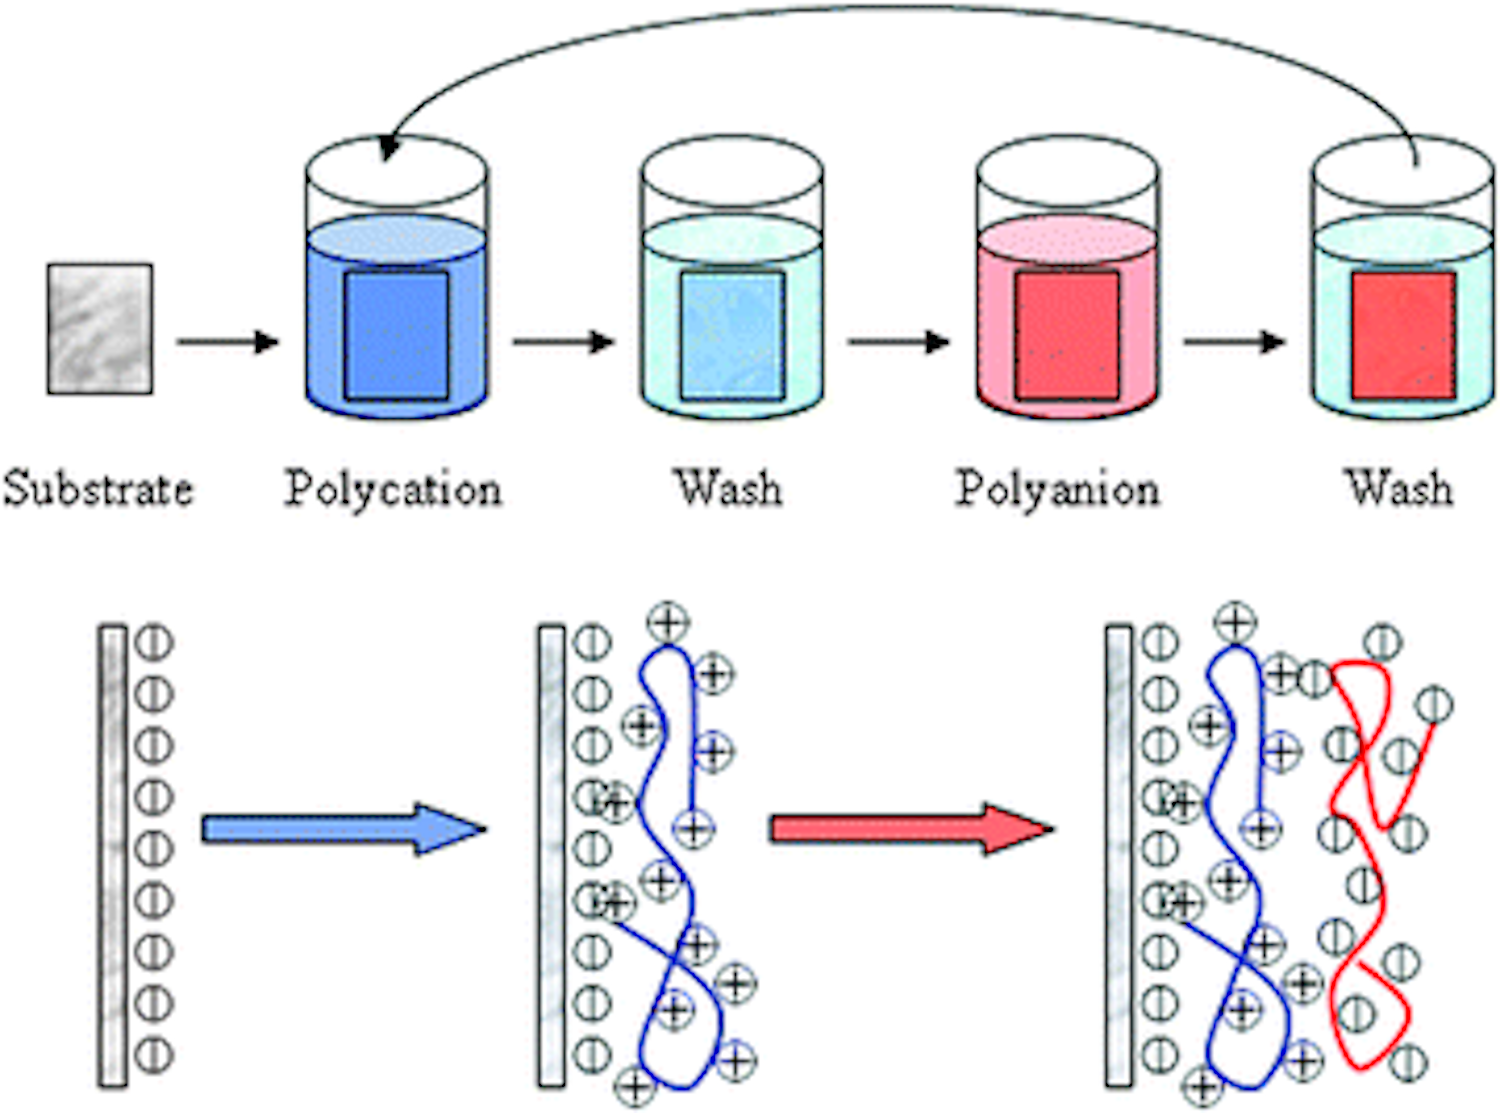
\includegraphics[width=0.9\columnwidth]{LBL}
	\caption{Scheme of sample preparation by LBL\cite{fig_LBL}.}
	\label{fig:lbl}
\end{figure}


\section{Results and discussion}

\subsection{Absorption spectra}


\begin{figure}[h!]
	\centering
	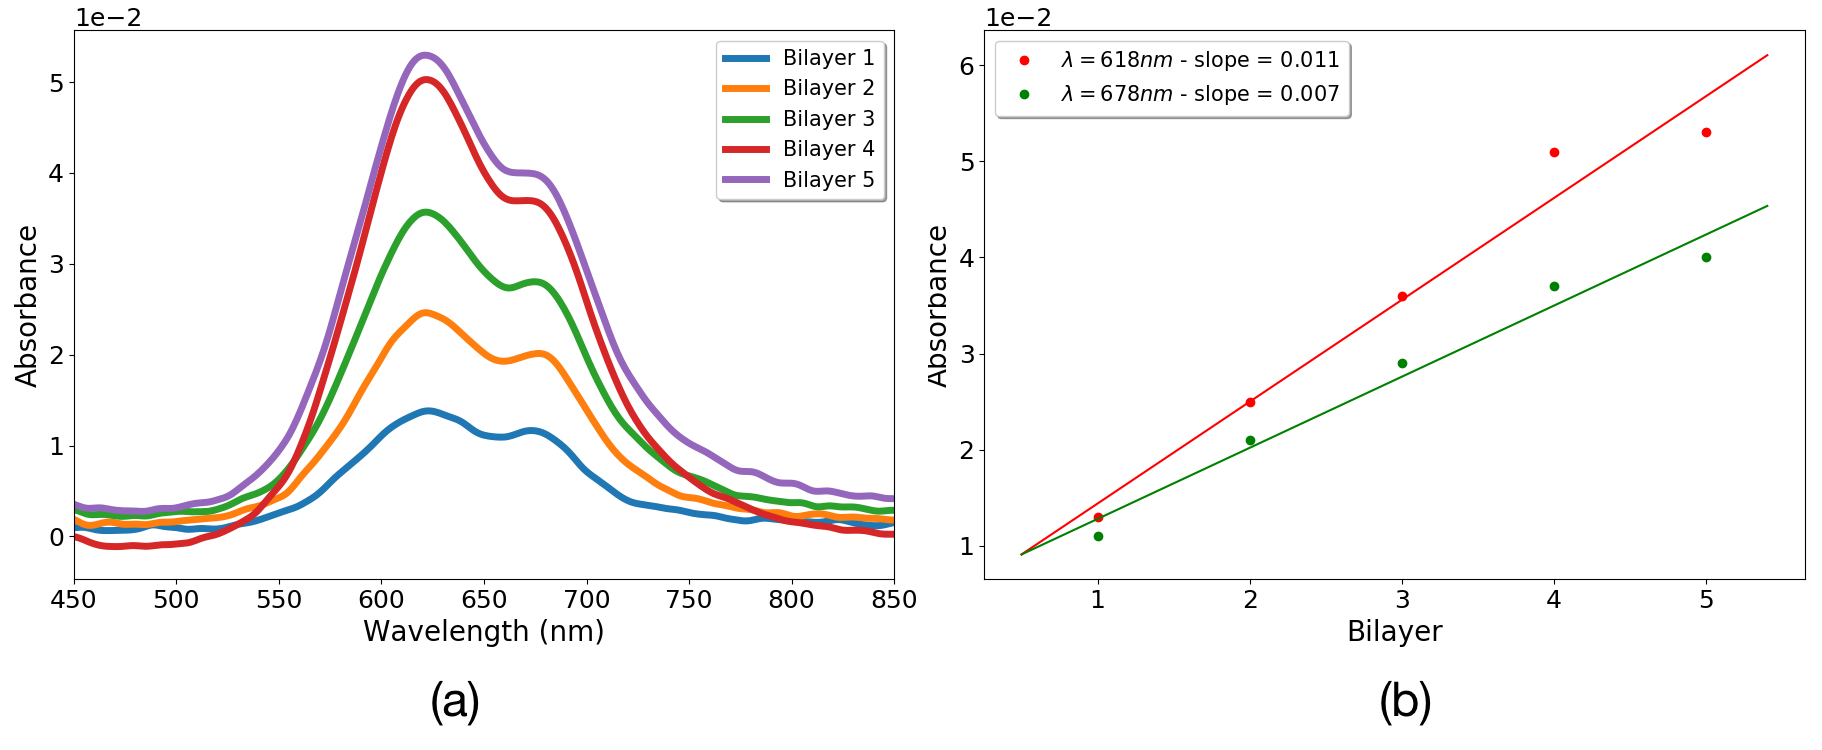
\includegraphics[width=\columnwidth]{uv}
	\caption{}
	\label{fig:rafael}
\end{figure}


\begin{figure}[h!]
	\centering
	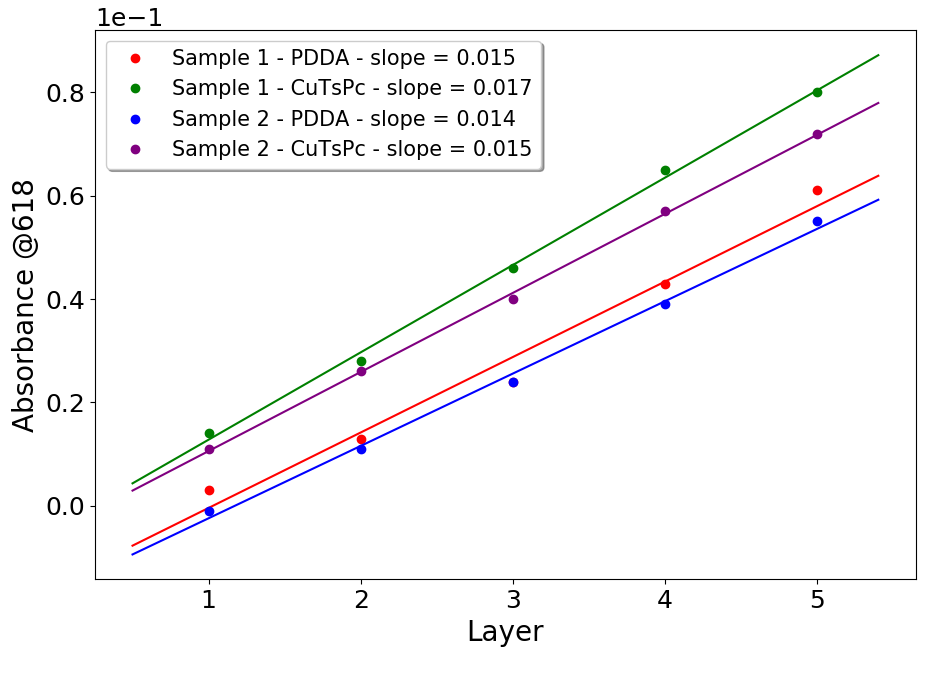
\includegraphics[width=0.8\columnwidth]{rafael}
	\caption{}
	\label{fig:rafael}
\end{figure}



\subsection{Atomic force microscopy}

Figure~\ref{fig:1} shows AFM images of the substrate before film deposition, for different scan sizes. Since the deposited film is very thin, we can compare AFM images of the substrate before and after deposition to verify the layers are being formed. We can also observe the surface is not completely flat from the images of figure~\ref{fig:1}, the RMS values calculated from figure~\ref{fig:1}(a) and (b) are (479 $\pm$ 24)pm and (413 $\pm$ 20)pm, respectively. 

\begin{figure}[h!]
	\centering
	\includegraphics[width=\columnwidth]{vidro}
	\caption{Atomic force microscopy images (topography) of the surface of the substrate (hydrophilized glass) before film deposition. Scale bar: (a) 1$\mu$m and (b) 500nm.}
	\label{fig:1}
\end{figure}

Figure~\ref{fig:3} shows AFM images of the substrate after the deposition of a film containing 15 bilayers of PDDA/CuTsPc. Figure~\ref{fig:3}(a) and (b) present the surface topography of an area 20 x 20 $\mu$m and 2 x 2 $\mu$m in dimension, respectively. This morphologic investigation shows a very uniform surface, the RMS values calculated from figure~\ref{fig:3}(a) and (b) are (5.0 $\pm$ 0.3)nm and (3.4 $\pm$ 0.2)nm, respectively. Comparing figure~\ref{fig:1}(b) and \ref{fig:3}(b), the topography indicates that the film is being deposited due to the change in topography, RMS values also shows changes for both cases.


\begin{figure}[h!]
	\centering
	\includegraphics[width=\columnwidth]{dipping}
	\caption{Atomic force microscopy images (topography) of the surface of the film (PDDA/CuTsPc) deposited by LBL. Scale bar: (a) 5$\mu$m and (b) 500nm.}
	\label{fig:3}
\end{figure}

Figure~\ref{fig:2}(a) shows an AFM image of a step in the deposited film. Using the topography image we were able to measure the film thickness, as shown in figure~\ref{fig:2}(b). The average thickness measured for the curves in figure~\ref{fig:2}(b) is $\bar{T}$=(33$\pm$2)nm. According to the literature, a mono layer of PDDA film has $\sim$1.7 nm thickness \cite{PDDA}, and a mono layer of CuTsPc has $\sim$0.6 nm \cite{Cu}. It is consistent to the thickness measured for our 15 PDDA/CuTsPc bilayer thickness, (33$\pm$2)nm. This indicates our method is actually forming mono layers in each part of the LBL process. 


\begin{figure}[h!]
	\centering
	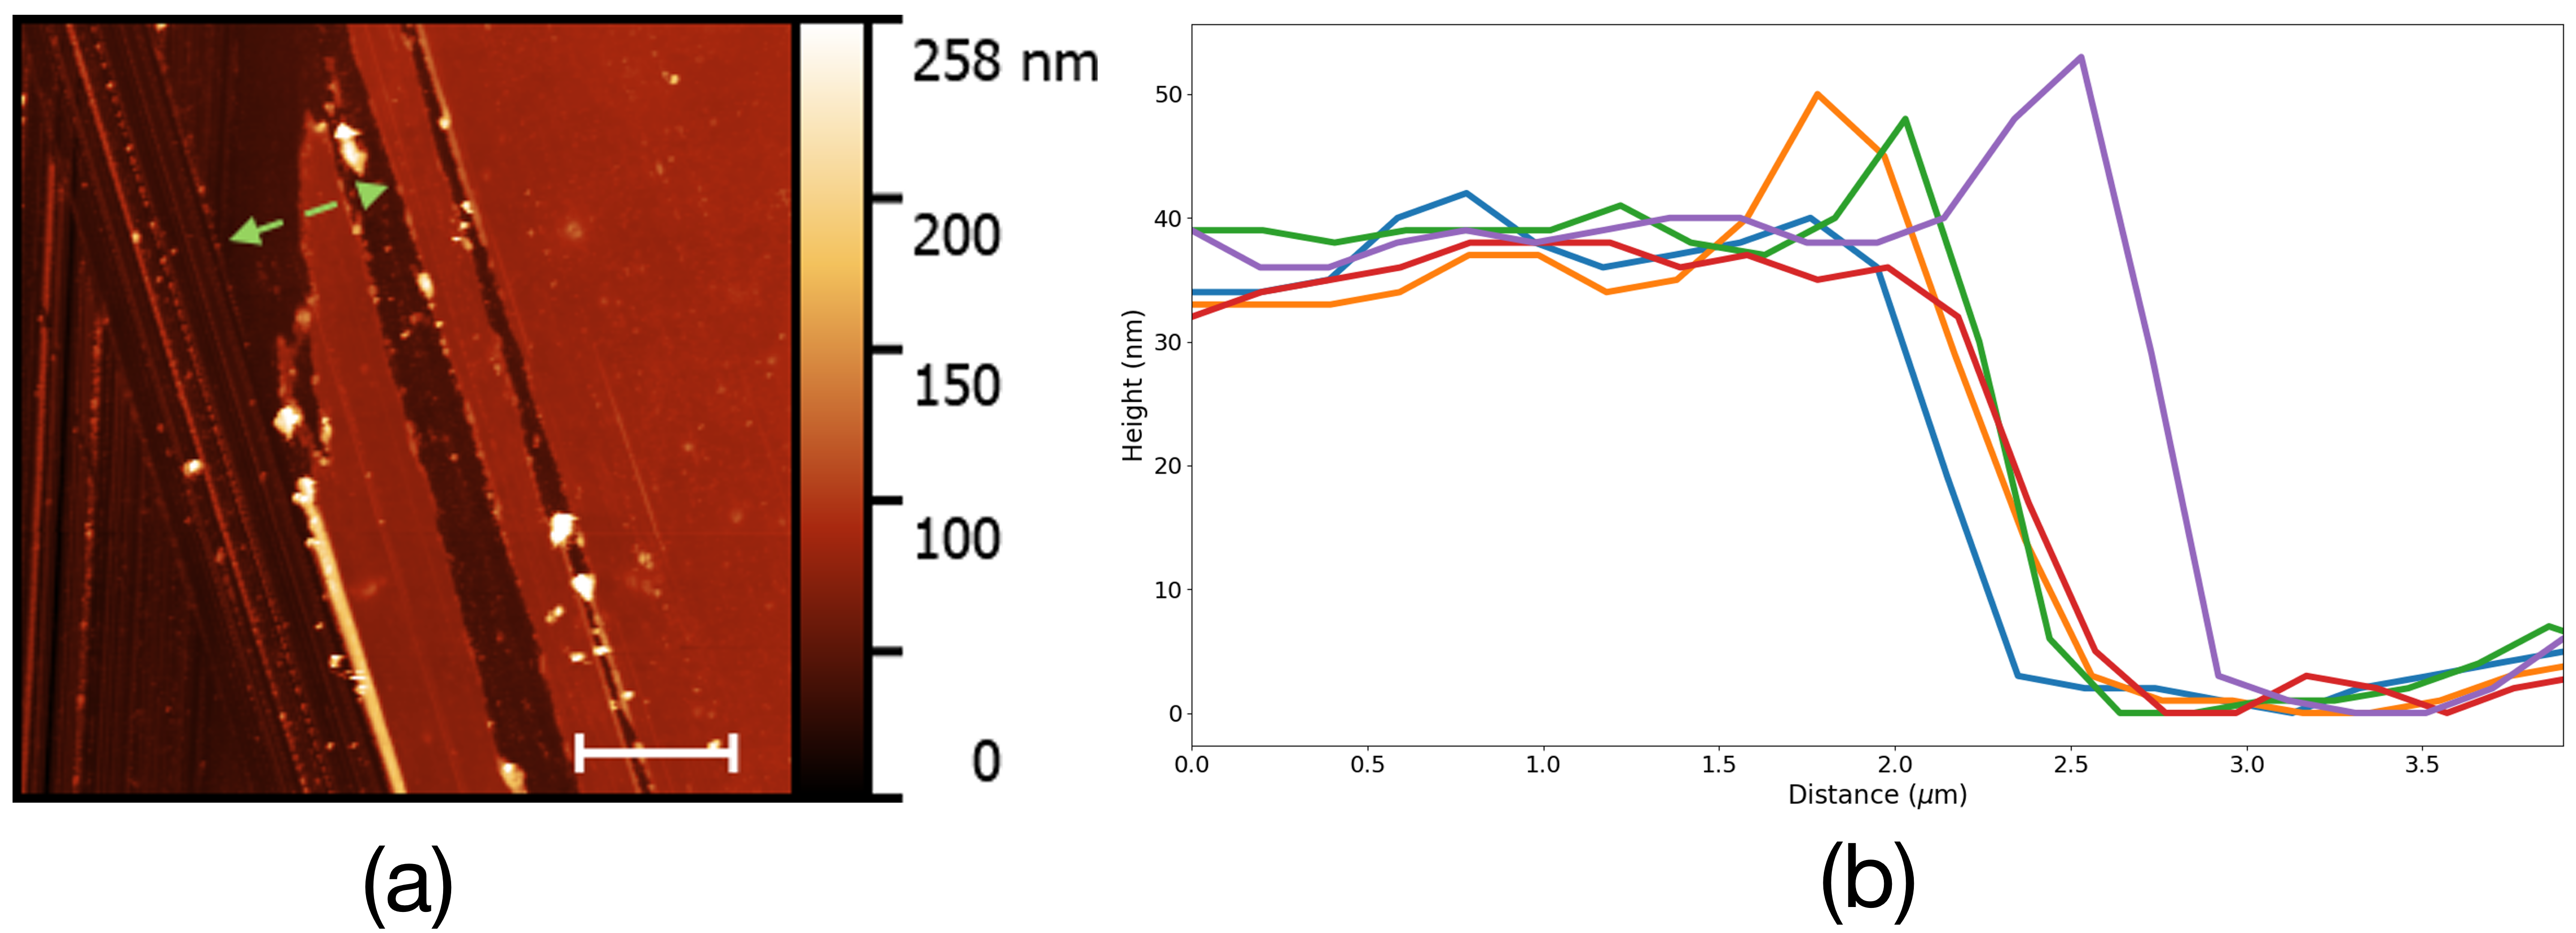
\includegraphics[width=0.98\columnwidth]{degrau1}
	\caption{(a) Atomic force microscopy image (topography) showing a step in the film deposited (PDDA/CuTsPc). Scale bar: 10$\mu$m. (b) Height profile of the step measured with the AFM.}
	\label{fig:2}
\end{figure}




\section{Conclusion}

\begin{thebibliography}{10}

\end{thebibliography}

%\bibliographystyle{nnn}
%\bibliography{/Users/marianazavarize/Dropbox/FI119/Artigo/bib.bib}

\end{document}
%
% ****** End of file apssamp.tex ******
